% !TeX program = xelatex
% 2025 年普通高等学校招生全国统一考试（新课标 I 卷）数学 —— 原卷版
% 编译方式：XeLaTeX，需要 exam-zh 宏包（TeX Live 2020+）
\documentclass{exam-zh}
\usepackage{tikz}
\usepackage{diagbox}
\examsetup{
  question/show-answer = false,
}

\begin{document}

\begin{center}
  {\zihao{3}\bfseries 2025 年普通高等学校招生全国统一考试（新课标 \uppercase\expandafter{\romannumeral1} 卷）}\\[4pt]
  {\zihao{4}\bfseries 数\quad 学}
\end{center}

\noindent\textbf{注意事项：}
\begin{enumerate}
  \item 答卷前，考生务必用黑色字迹的钢笔或签字笔将自己的姓名和考生号、试室号、座位号填写在答题卡上。用 2B 铅笔将试卷类型和考生号填涂在答题卡相应位置上。
  \item 选择题每小题选出答案后，用 2B 铅笔把答题卡上对应的题目选项的答案信息点涂黑；如需改动，用橡皮擦干净后，再填涂其他答案。答案不能答在试卷上。
  \item 非选择题必须用黑色字迹的钢笔或签字笔作答，答案必须写在答题卡各题目指定区域内相应位置上；如需改动，先划掉原来的答案，然后再写上新的答案，不准使用铅笔和涂改液。不按以上要求作答的答案无效。
\end{enumerate}

\section{选择题：本题共 8 小题，每小题 5 分，共 40 分。在每小题给出的四个选项中，只有一项是符合题目要求的。}

\begin{question}
$(1+5\iu)\iu$ 的虚部为 \paren
\begin{choices}
  \item $-1$
  \item $0$
  \item $1$
  \item $6$
\end{choices}
\end{question}

\begin{question}
设全集 $U=\{x\mid x\text{ 是小于 }9\text{ 的正整数}\}$，集合 $A=\{1,3,5\}$，则 $\complement_{U}A$ 中元素个数为 \paren
\begin{choices}
  \item $0$
  \item $3$
  \item $5$
  \item $8$
\end{choices}
\end{question}

\begin{question}
若双曲线 $C$ 的虚轴长为实轴长的 $\sqrt{7}$ 倍，则 $C$ 的离心率为 \paren
\begin{choices}
  \item $\sqrt{2}$
  \item $2$
  \item $\sqrt{7}$
  \item $2\sqrt{2}$
\end{choices}
\end{question}

\begin{question}
若点 $(a,0)\,(a>0)$ 是函数 $y=2\tan\left(x-\dfrac{\uppi}{3}\right)$ 的图象的一个对称中心，则 $a$ 的最小值为 \paren
\begin{choices}
  \item $\dfrac{\uppi}{4}$
  \item $\dfrac{\uppi}{2}$
  \item $\dfrac{\uppi}{3}$
  \item $\dfrac{4\uppi}{3}$
\end{choices}
\end{question}

\begin{question}
设 $f(x)$ 是定义在 $\mathbb{R}$ 上且周期为 $2$ 的偶函数，当 $2\le x\le 3$ 时，$f(x)=5-2x$，则 $f\left(-\dfrac{3}{4}\right)=$ \paren
\begin{choices}
  \item $-\dfrac{1}{2}$
  \item $-\dfrac{1}{4}$
  \item $\dfrac{1}{4}$
  \item $\dfrac{1}{2}$
\end{choices}
\end{question}

\begin{question}
帆船比赛中，运动员可借助风力计测定风速的大小和方向，测出的结果在航海学中称为视风速。视风速对应的向量，是真风速对应的向量与船行风速对应的向量之和，其中船行风速对应的向量与船速对应的向量大小相同，方向相反。图 1 给出了部分风力等级、名称与风速大小的对应关系。已知某帆船运动员在某时刻测得的视风风速对应的向量与船速对应的向量如图 2（风速的大小和向量的大小相同），单位（m/s），则真风为 \paren

\begin{center}
\begin{tabular}{|c|c|c|}
\hline
等级 & 风速大小 m/s & 名称 \\
\hline
2 & $1.1\sim 3.3$ & 轻风 \\
\hline
3 & $3.4\sim 5.4$ & 微风 \\
\hline
4 & $5.5\sim 7.9$ & 和风 \\
\hline
5 & $8.0\sim 10.1$ & 劲风 \\
\hline
\end{tabular}

\vspace{4pt}
{\footnotesize 图 1}
\end{center}

\begin{center}
\begin{tikzpicture}[scale=0.9,>=stealth]
  \draw[->](0,0)--(4,0)node[right]{$x$};
  \draw[->](0,0)--(0,4)node[above]{$y$};
  \foreach \i in {1,2,3}{
    \draw(\i,0.08)--(\i,-0.08)node[below]{\scriptsize$\i$};
    \draw(0.08,\i)--(-0.08,\i)node[left]{\scriptsize$\i$};}
  \draw[->,very thick](0,0)--(3,3);
  \node at (1.15,2.15){\footnotesize 视风风速};
  \draw[->,very thick](2,1)--(3,3);
  \node at (2.75,1.55){\footnotesize 船速};
  \draw[dashed](2,0)--(2,1)--(0,1);
  \node[below] at (0,-0.15){\scriptsize $O$};
  \node at (1.7,-0.6){\footnotesize 图 2};
\end{tikzpicture}
\end{center}

\begin{choices}
  \item 轻风
  \item 微风
  \item 和风
  \item 劲风
\end{choices}
\end{question}

\begin{question}
若圆 $x^{2}+(y+2)^{2}=r^{2}\,(r>0)$ 上到直线 $y=\sqrt{3}x+2$ 的距离为 $1$ 的点有且仅有 $2$ 个，则 $r$ 的取值范围是 \paren
\begin{choices}
  \item $(0,1)$
  \item $(1,3)$
  \item $(3,+\infty)$
  \item $(0,+\infty)$
\end{choices}
\end{question}

\begin{question}
若实数 $x,y,z$ 满足 $2+\log_{2}x=3+\log_{3}y=5+\log_{5}z$，则 $x,y,z$ 的大小关系不可能是 \paren
\begin{choices}
  \item $x>y>z$
  \item $x>z>y$
  \item $y>x>z$
  \item $y>z>x$
\end{choices}
\end{question}

\section{选择题：本题共 3 小题，每小题 6 分，共 18 分。在每小题给出的选项中，有多项符合题目要求。全部选对的得 6 分，部分选对的得部分分，有选错的得 0 分。}

\begin{question}
在正三棱柱 $ABC\text{-}A_{1}B_{1}C_{1}$ 中，$D$ 为 $BC$ 中点，则 \paren
\begin{choices}
  \item $AD\perp A_{1}C$
  \item $BC\perp$ 平面 $AA_{1}D$
  \item $CC_{1}\parallel$ 平面 $AA_{1}D$
  \item $AD\parallel A_{1}B_{1}$
\end{choices}
\end{question}

\begin{question}
设抛物线 $C\colon y^{2}=6x$ 的焦点为 $F$，过 $F$ 的直线交 $C$ 于 $A$、$B$，过 $F$ 且垂直于 $AB$ 的直线交 $l\colon x=-\dfrac{3}{2}$ 于 $E$，过点 $A$ 作准线 $l$ 的垂线，垂足为 $D$，则 \paren
\begin{choices}
  \item $|AD|=|AF|$
  \item $|AE|=|AB|$
  \item $|AB|\ge 6$
  \item $|AE|\cdot|BE|\ge 18$
\end{choices}
\end{question}

\begin{question}
已知 $\triangle ABC$ 的面积为 $\dfrac{1}{4}$，若 $\cos 2A+\cos 2B+2\sin C=2$，$\cos A\cos B\sin C=\dfrac{1}{4}$，则 \paren
\begin{choices}
  \item $\sin C=\sin^{2}A+\sin^{2}B$
  \item $AB=\sqrt{2}$
  \item $\sin A+\sin B=\dfrac{\sqrt{6}}{2}$
  \item $AC^{2}+BC^{2}=3$
\end{choices}
\end{question}

\section{填空题：本题共 3 小题，每小题 5 分，共 15 分。}

\begin{question}
若直线 $y=2x+5$ 是曲线 $y=\eu^{x}+x+a$ 的切线，则 $a=$ \fillin 。
\end{question}

\begin{question}
若一个等比数列的前 $4$ 项和为 $4$，前 $8$ 项和为 $68$，则该等比数列的公比为 \fillin 。
\end{question}

\begin{question}
一个箱子里有 $5$ 个相同的球，分别以 $1\sim 5$ 标号，若有放回地取三次，记至少取出一次的球的个数 $X$，则数学期望 $E(X)=$ \fillin 。
\end{question}

\section{解答题：本题共 5 小题，共 77 分。解答应写出文字说明、证明过程或演算步骤。}

\begin{problem}[points = 13]
为研究某疾病与超声波检查结果的关系，从做过超声波检查的人群中随机调查了 $1000$ 人，得到如下列联表：

\begin{center}
\begin{tabular}{|c|c|c|c|}
\hline
\diagbox{组别}{超声波检查结果} & 正常 & 不正常 & 合计 \\
\hline
患该疾病 & $20$ & $180$ & $200$ \\
\hline
未患该疾病 & $780$ & $20$ & $800$ \\
\hline
合计 & $800$ & $200$ & $1000$ \\
\hline
\end{tabular}
\end{center}

（1）记超声波检查结果不正常者患该疾病的概率为 $P$，求 $P$ 的估计值；

（2）根据小概率值 $\alpha=0.001$ 的独立性检验，分析超声波检查结果是否与患该疾病有关。

附 $\chi^{2}=\dfrac{n(ad-bc)^{2}}{(a+b)(c+d)(a+c)(b+d)}$，

\begin{center}
\begin{tabular}{|c|c|c|c|}
\hline
$P(\chi^{2}\ge k)$ & $0.050$ & $0.010$ & $0.001$ \\
\hline
$k$ & $3.841$ & $6.635$ & $10.828$ \\
\hline
\end{tabular}
\end{center}
\end{problem}

\begin{problem}[points = 15]
设数列 $\{a_{n}\}$ 满足 $a_{1}=3$，$\dfrac{a_{n+1}}{n}=\dfrac{a_{n}}{n+1}+\dfrac{1}{n(n+1)}$。

（1）证明：$\{na_{n}\}$ 为等差数列；

（2）设 $f(x)=a_{1}x+a_{2}x^{2}+\cdots+a_{m}x^{m}$，求 $f'(-2)$。
\end{problem}

\begin{problem}[points = 15]
如图所示的四棱锥 $P\text{-}ABCD$ 中，$PA\perp$ 平面 $ABCD$，$BC\parallel AD$，$AB\perp AD$。

\begin{center}
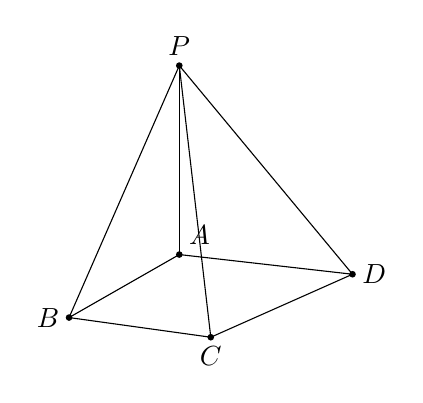
\begin{tikzpicture}[scale=1.0,>=stealth]
  \coordinate (A) at (0,0);
  \coordinate (B) at (-1.4,-0.8);
  \coordinate (C) at (0.4,-1.05);
  \coordinate (D) at (2.2,-0.25);
  \coordinate (P) at (0,2.4);
  \draw (A)--(B)--(C)--(D)--(A);
  \draw (P)--(A); \draw (P)--(B); \draw (P)--(C); \draw (P)--(D);
  \foreach \pt/\pos in {A/{above right},B/{left},C/{below},D/{right},P/{above}}
    \fill (\pt) circle (1.2pt) node[\pos]{$\pt$};
\end{tikzpicture}
\end{center}

（1）证明：平面 $PAB\perp$ 平面 $PAD$；

（2）$PA=AB=\sqrt{2}$，$AD=1+\sqrt{3}$，$BC=2$，$P$、$B$、$C$、$D$ 在同一个球面上，设该球面的球心为 $O$。

\qquad（i）证明：$O$ 在平面 $ABCD$ 上；

\qquad（ii）求直线 $AC$ 与直线 $PO$ 所成角的余弦值。
\end{problem}

\begin{problem}[points = 17]
设椭圆 $C\colon \dfrac{x^{2}}{a^{2}}+\dfrac{y^{2}}{b^{2}}=1\,(a>b>0)$ 的离心率为 $\dfrac{2\sqrt{2}}{3}$，下顶点为 $A$，右顶点为 $B$，$|AB|=\sqrt{10}$。

（1）求椭圆的标准方程；

（2）已知点 $P$ 不在 $y$ 轴上，点 $R$ 在射线 $AP$ 上，且满足 $|AR|\cdot|AP|=3$。

\qquad（i）设 $P(m,n)$，求点 $R$ 的坐标（用 $m$、$n$ 表示）；

\qquad（ii）设 $O$ 为坐标原点，$M$ 是椭圆上的动点，直线 $OR$ 的斜率是直线 $OP$ 的斜率的 $3$ 倍，求 $|PM|$ 的最大值。
\end{problem}

\begin{problem}[points = 17]
设函数 $f(x)=5\cos x-\cos 5x$。

（1）求 $f(x)$ 在 $\left[0,\dfrac{\uppi}{4}\right]$ 的最大值；

（2）给定 $\theta\in(0,\uppi)$，设 $a$ 为实数，证明：存在 $y\in[a-\theta,a+\theta]$，使得 $\cos y\le\cos\theta$；

（3）若存在 $\varphi$ 使得对任意 $x$，都有 $5\cos x-\cos(5x+\varphi)\le b$，求 $b$ 的最小值。
\end{problem}

\end{document}
